\begin{figure}[t]
  \centering
  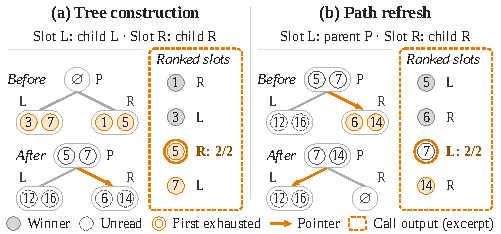
\includegraphics[width=\linewidth]{fig/mechanisms/pointer.pdf}
  \caption{Pointer assignment ($h=2$). The first slot to supply its second entry in the replay order determines the pointer. In (a), R reaches that entry at row 5. In (b), the old parent segment occupies L and reaches its second entry at row 7. L and R are slot labels, not the original run identities.}
  \label{fig:pointer-mechanism}
\end{figure}
